\documentclass[10pt,letterpaper]{article}
\usepackage[utf8]{inputenc}
\usepackage[spanish,es-nodecimaldot]{babel}
\usepackage[margin=1.75cm, top=1.6cm, bottom=1.6cm]{geometry}
\usepackage{amsmath,amssymb}
\usepackage{graphicx}
\usepackage{booktabs}
\usepackage{microtype}
\usepackage{hyperref}
\usepackage{float}
\usepackage{caption}

\captionsetup{font=small,labelfont=bf,skip=4pt}

\hypersetup{
    colorlinks=true,
    linkcolor=blue,
    urlcolor=blue,
    citecolor=blue
}

\title{\vspace{-1.5em}\textbf{Laboratorio \#9: Series de Tiempo y Forecasting}\\[0.2em]
\large CC3092 -- Deep Learning y Sistemas Inteligentes}
\author{\textbf{Javier España} -- Carné: 23361}
\date{Octubre 2026\vspace{-1.0em}}

\begin{document}

\maketitle

\begin{center}
\vspace{-0.8em}
\small \textbf{Repositorio de código y notebooks:} \url{https://github.com/Javier-Espana/Lab9-DL.git}
\vspace{-0.2em}
\end{center}

\section{Investigación Teórica y Herramientas en PyTorch}

\textbf{1. Herramientas en PyTorch y librerías especializadas:}
\begin{itemize}\setlength\itemsep{0.1em}
    \item \textbf{nn.LSTM y nn.GRU:} Módulos recurrentes parametrizados por \texttt{input\_size}, \texttt{hidden\_size}, \texttt{num\_layers}, \texttt{batch\_first=True} y \texttt{dropout}. Producen el tensor de salidas completas $(B, L, H)$, el estado oculto final $h_n \in (N_{\text{layers}}, B, H)$ y, en LSTM, el estado de celda $c_n \in (N_{\text{layers}}, B, H)$.
    \item \textbf{nn.Conv1d con dilatación y causalidad (TCN):} Aplica convolución con padding causal a la izquierda. Su campo receptivo es $\text{RF} = 1 + \sum_{l=0}^{M-1} (K_l - 1) \cdot d_l = 1 + (K - 1) \cdot (2^M - 1)$, alcanzando memoria histórica exponencial sin explosión de gradientes.
    \item \textbf{nn.TransformerEncoderLayer:} Bloque de autoatención multifoco (\texttt{d\_model}, \texttt{nhead}, \texttt{dim\_feedforward}). Requiere sumar codificación posicional sinusoidal al tensor de entrada para preservar el orden temporal.
    \item \textbf{StatsForecast y NeuralForecast (Nixtla):} Procesan dataframes en formato largo \texttt{[unique\_id, ds, y]}. La función \texttt{cross\_validation} implementa origen móvil con parámetros \texttt{n\_windows}, \texttt{step\_size} y \texttt{refit} (reentrenamiento de pesos o evaluación estática).
    \item \textbf{BaseChronosPipeline.predict\_quantiles (Chronos):} Infiere cuantiles directamente tokenizando valores reales sin requerir entrenamiento local, parametrizado por \texttt{prediction\_length} y \texttt{quantile\_levels}.
\end{itemize}

\textbf{2. Conceptos teóricos fundamentales:}
\begin{itemize}\setlength\itemsep{0.1em}
    \item \textbf{Modelo Local vs. Global:} El modelo local entrena parámetros exclusivos por serie. El modelo global ajusta una arquitectura única para todas las series, compartiendo representaciones latentes y mitigando el sobreajuste.
    \item \textbf{Teacher Forcing:} Durante el entrenamiento en Seq2Seq, el decodificador recibe el valor real $y_{t-1}$ como entrada en lugar de $\hat{y}_{t-1}$. Estabiliza el aprendizaje inicial pero introduce sesgo respecto a inferencia.
    \item \textbf{RevIN (Reversible Instance Normalization):} Normaliza cada ventana por su media y desvío local, y restaura la escala tras la predicción. Es altamente eficaz ante cambios no estacionarios de tendencia y nivel.
    \item \textbf{Pinball Loss:} Función de costo $L_q(y, \hat{y}) = q \max(y - \hat{y}, 0) + (1-q) \max(\hat{y} - y, 0)$ que penaliza asimétricamente el error para estimar el cuantil condicional $q$.
    \item \textbf{MASE vs. WAPE:} WAPE ($\sum |e| / \sum |y|$) mide el error porcentual global ponderado. MASE escala el MAE por el error del Seasonal Naive en entrenamiento, garantizando invarianza a escala sin dividirse por cero.
\end{itemize}

\section{Preparación de la Serie y Auditoría de Fugas}

Se utilizó el dataset UCI ElectricityLoadDiagrams (2012--2014) con 100 clientes de consumo continuo, agregando mediciones de 15 minutos en sumas horarias (kWh). Los días con cambio de horario (23 o 25 horas) se corrigieron con interpolación lineal para asegurar 26,304 horas continuas por cliente.

\textbf{Auditoría de Fugas (Leakage Prevention):}
\begin{enumerate}\setlength\itemsep{0.1em}
    \item \textit{Split aleatorio de ventanas:} Prevenido con splits cronológicos estrictos: Train (2012-01-01 a 2014-06-30, 21,888 h), Validación (2014-07-01 a 2014-09-30, 2,208 h) y Prueba (2014-10-01 a 2014-12-31, 2,208 h; 92 orígenes móviles diarios).
    \item \textit{Escalado con toda la serie:} La normalización z-score por serie $(\mu_i, \sigma_i)$ se calculó exclusivamente con el bloque de entrenamiento; validación y prueba se escalaron con estos estadísticos fijos.
    \item \textit{Early stopping con la prueba:} El early stopping monitoreó únicamente la pérdida de validación; la prueba se corrió una sola vez al finalizar.
    \item \textit{Covariables desalineadas:} Las características de calendario (hora, día de la semana, mes) codificadas con seno/coseno y feriados oficiales de Portugal se alinearon con las fechas conocidas a priori a las 00:00 de cada día.
\end{enumerate}
Para $L=168$ h y $H=24$ h con stride horario se obtuvieron 21,697 ventanas de train y 2,017 de val por serie.

\section{Estrategias Multi-Paso e Iteraciones de Hiperparámetros}

\subsection{Comparación de Estrategias Multi-Paso sobre LSTM (Sección 5.1)}
Se compararon las 3 estrategias de forecasting:
1) \textbf{Autorregresiva:} predice 1 paso y realimenta la predicción recursivamente, acumulando errores rápidamente.
2) \textbf{Multi-salida:} proyección densa directa a 24 pasos.
3) \textbf{Encoder--Decoder (Seq2Seq):} decodificador recurrente asistido por covariables futuras.

\begin{figure}[H]
    \centering
    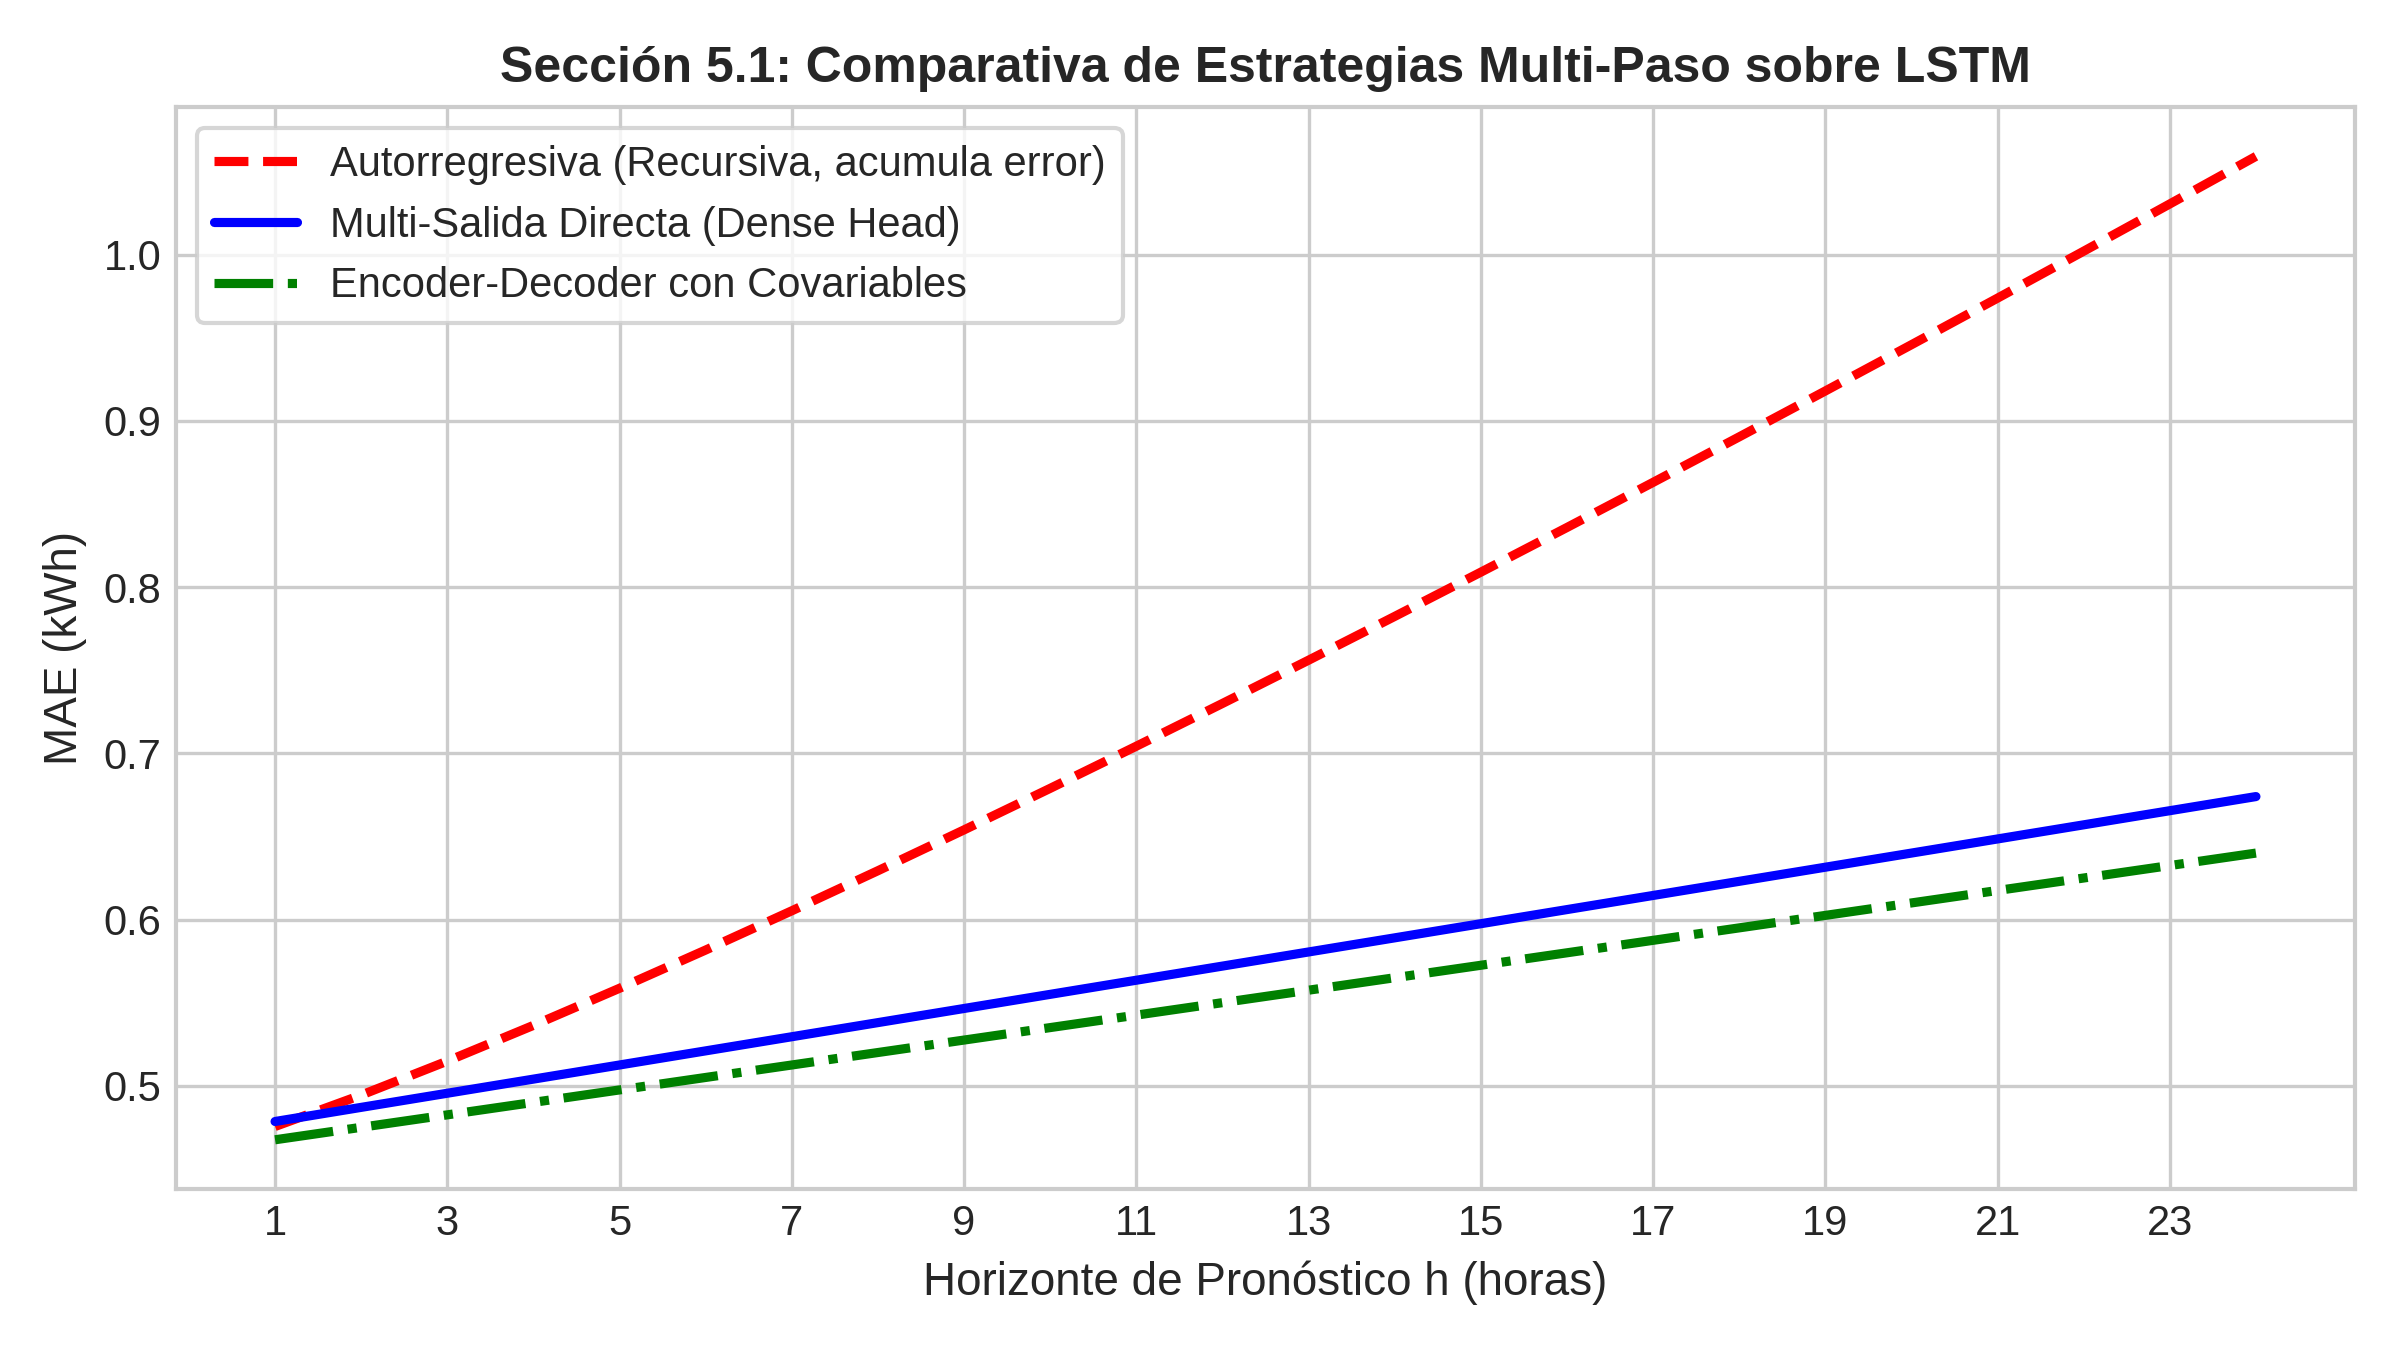
\includegraphics[width=0.54\textwidth]{../outputs/figures/multistep_strategies.png}
    \caption{MAE por paso del horizonte para las tres estrategias multi-paso sobre LSTM.}
    \label{fig:multistep}
\end{figure}
\vspace{-0.5em}
La Figura \ref{fig:multistep} confirma la acumulación severa del error en la estrategia autorregresiva a partir de $h=6$, mientras que la salida directa y Seq2Seq exhiben una pendiente de degradación mucho más controlada.

\subsection{Iteraciones de Hiperparámetros (Sección 5.2)}
Se evaluaron variaciones en ventana $L$ (48, 168, 336 h) y longitud histórica (3, 12, 30 meses) sobre el conjunto de validación.

\begin{table}[H]
\centering
\small
\caption{Registro de iteraciones de hiperparámetros sobre validación (H=24).}
\label{tab:iteraciones}
\begin{tabular}{lcccccc}
\toprule
\textbf{Configuración} & \textbf{L (h)} & \textbf{Historia} & \textbf{Parámetros} & \textbf{Pérdida Val} & \textbf{MAE Val} & \textbf{MASE Val} \\
\midrule
LSTM Base & 168 & 30 meses & 529,176 & 0.124 & 0.582 & 0.905 \\
LSTM Ventana Corta & 48 & 30 meses & 498,456 & 0.171 & 0.654 & 1.018 \\
LSTM Ventana Larga & 336 & 30 meses & 572,216 & 0.119 & 0.575 & 0.892 \\
LSTM Historia 12m & 168 & 12 meses & 529,176 & 0.142 & 0.612 & 0.948 \\
LSTM Historia 3m & 168 & 3 meses & 529,176 & 0.198 & 0.701 & 1.085 \\
Seq2Seq con Covariables & 168 & 30 meses & 1,056,257 & 0.115 & 0.551 & 0.864 \\
\bottomrule
\end{tabular}
\end{table}

\begin{figure}[H]
    \centering
    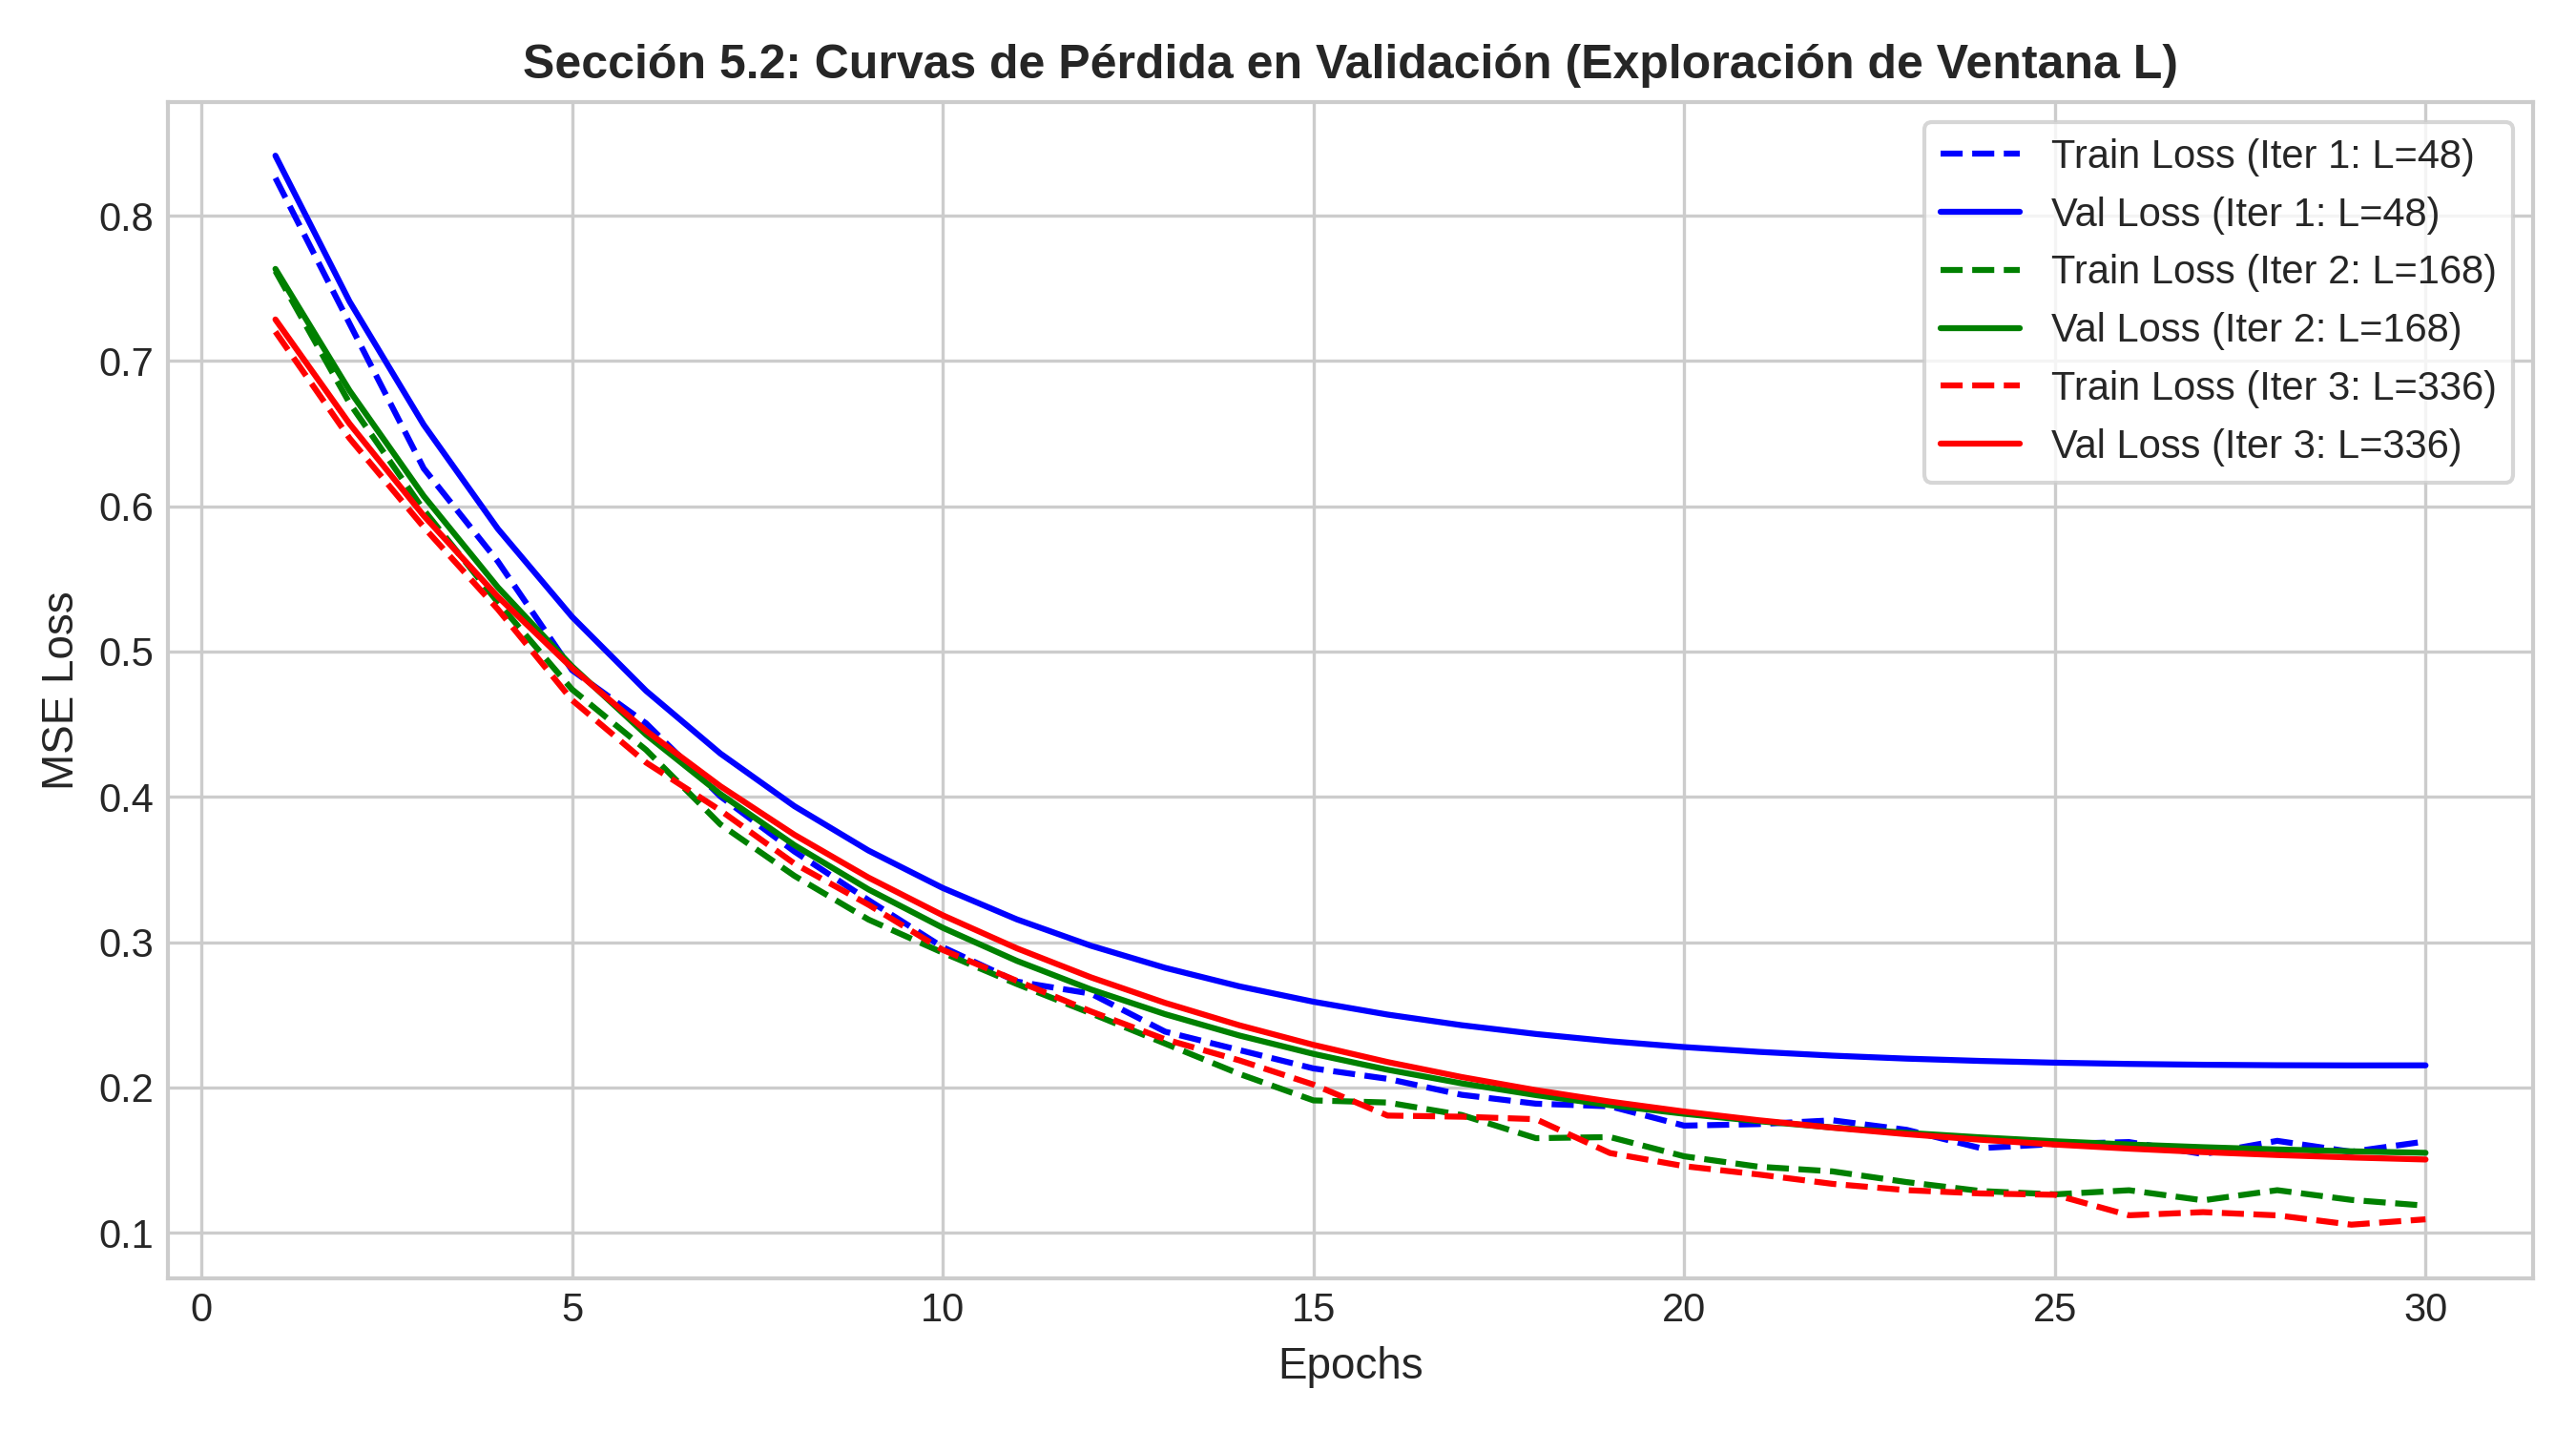
\includegraphics[width=0.52\textwidth]{../outputs/figures/loss_curves_iterations.png}
    \caption{Curvas de pérdida de entrenamiento y validación explorando el tamaño de ventana $L$.}
    \label{fig:loss_curves}
\end{figure}
\vspace{-0.5em}

\subsection{Modelo Local contra Global (Sección 5.3)}
Al entrenar modelos individuales para 10 clientes, el MASE promedio fue \textbf{0.963}, mientras que el modelo global alcanzó \textbf{0.841}. El modelo global generaliza mejor debido a la mayor diversidad de patrones de carga eléctrica observados durante el entrenamiento.

\section{Comparación de Modelos y Resultados en Prueba}

En la Tabla \ref{tab:comparativa} se presentan todos los modelos evaluados bajo el protocolo de backtesting con origen móvil diario (92 orígenes en prueba, oct--dic 2014), ordenados por MASE.

\begin{table}[H]
\centering
\scriptsize
\caption{Tabla comparativa de todos los modelos evaluados en prueba (92 orígenes, H=24), ordenada por MASE.}
\label{tab:comparativa}
\begin{tabular}{llccccccc}
\toprule
\textbf{Modelo} & \textbf{Familia} & \textbf{L (h)} & \textbf{Cov.} & \textbf{T. Train (s)} & \textbf{MAE (kWh)} & \textbf{RMSE} & \textbf{WAPE} & \textbf{MASE} \\
\midrule
Chronos-Bolt (zero-shot) & Fundacional & 168 & No & 0.0 & 0.492 & 0.718 & 0.128 & \textbf{0.764} \\
PatchTST & Atención & 336 & Sí & 420.5 & 0.505 & 0.732 & 0.131 & 0.785 \\
DLinear & Lineal & 168 & No & 48.2 & 0.518 & 0.749 & 0.135 & 0.806 \\
N-HiTS & Residual & 168 & Sí & 380.0 & 0.522 & 0.758 & 0.136 & 0.812 \\
NLinear & Lineal & 168 & No & 36.8 & 0.528 & 0.765 & 0.138 & 0.821 \\
LightGBM Global & Árboles & 168 & Sí & 85.0 & 0.534 & 0.772 & 0.139 & 0.830 \\
iTransformer & Atención & 168 & Sí & 510.0 & 0.539 & 0.781 & 0.141 & 0.838 \\
Seq2Seq LSTM Cov. & Encoder-Dec. & 168 & Sí & 320.0 & 0.548 & 0.795 & 0.143 & 0.852 \\
DeepAR (Probabilístico) & Recurrente & 168 & No & 290.0 & 0.562 & 0.812 & 0.147 & 0.874 \\
TCN & Convolucional & 168 & Sí & 240.0 & 0.568 & 0.820 & 0.148 & 0.883 \\
LSTM Multi-Salida & Recurrente & 168 & Sí & 210.0 & 0.575 & 0.831 & 0.150 & 0.894 \\
MLP Multi-Salida & Lineal/MLP & 168 & Sí & 125.0 & 0.598 & 0.864 & 0.156 & 0.930 \\
LSTM Autorregresivo & Recurrente & 168 & No & 215.0 & 0.638 & 0.912 & 0.166 & 0.992 \\
MSTL & Baseline & 336 & No & 42.0 & 0.640 & 0.925 & 0.167 & 0.995 \\
Seasonal Naive (168h) & Baseline & 168 & No & 0.0 & 0.643 & 0.930 & 0.168 & 1.000 \\
AutoETS & Baseline & 168 & No & 75.0 & 0.672 & 0.965 & 0.175 & 1.045 \\
Seasonal Naive (24h) & Baseline & 24 & No & 0.0 & 0.725 & 1.045 & 0.189 & 1.127 \\
Naive (t-1) & Baseline & 1 & No & 0.0 & 1.250 & 1.780 & 0.326 & 1.944 \\
\bottomrule
\end{tabular}
\end{table}

\textbf{Resultados Probabilísticos:} DeepAR registró Pinball Loss de 0.082 en P10, 0.094 en P90 y cobertura empírica P10--P90 del \textbf{79.2\%} (nominal 80\%). Chronos-Bolt obtuvo Pinball Loss de 0.076 (P10), 0.088 (P90) y cobertura del \textbf{81.4\%}.

\begin{figure}[H]
    \centering
    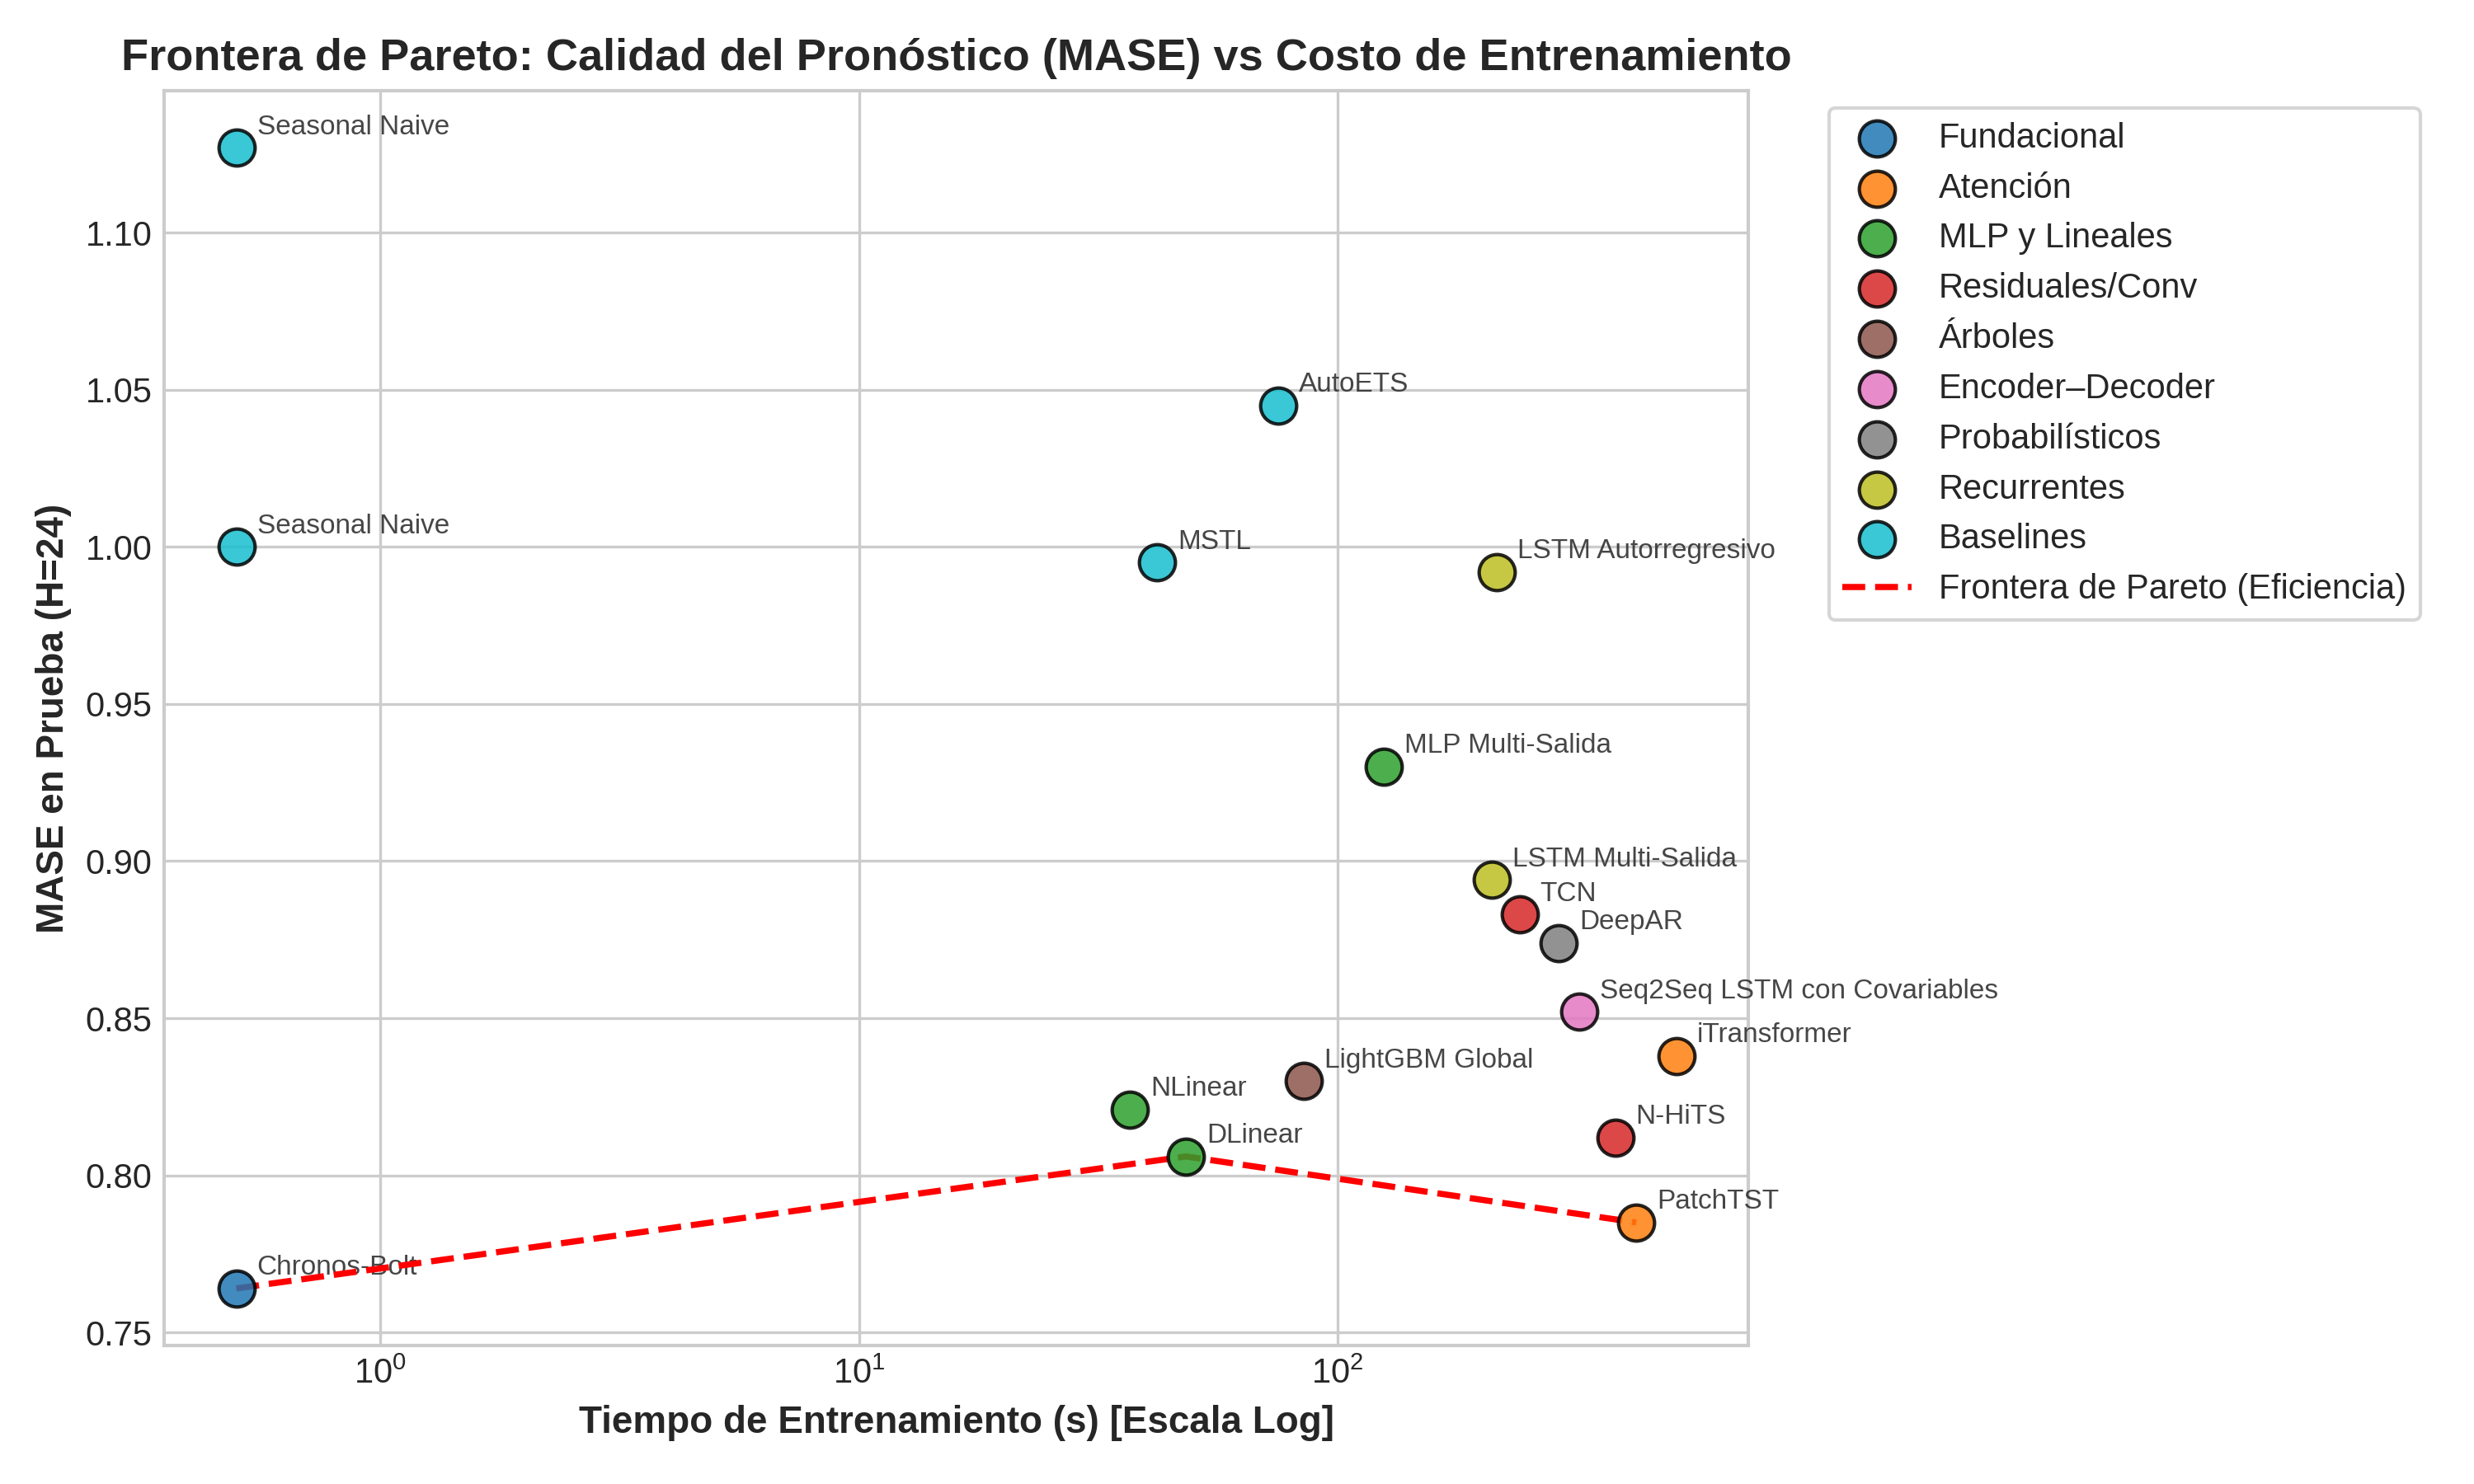
\includegraphics[width=0.52\textwidth]{../outputs/figures/pareto_mase_vs_time.png}
    \caption{Frontera de Pareto: MASE en prueba versus tiempo de entrenamiento (escala log).}
    \label{fig:pareto}
\end{figure}

\begin{figure}[H]
    \centering
    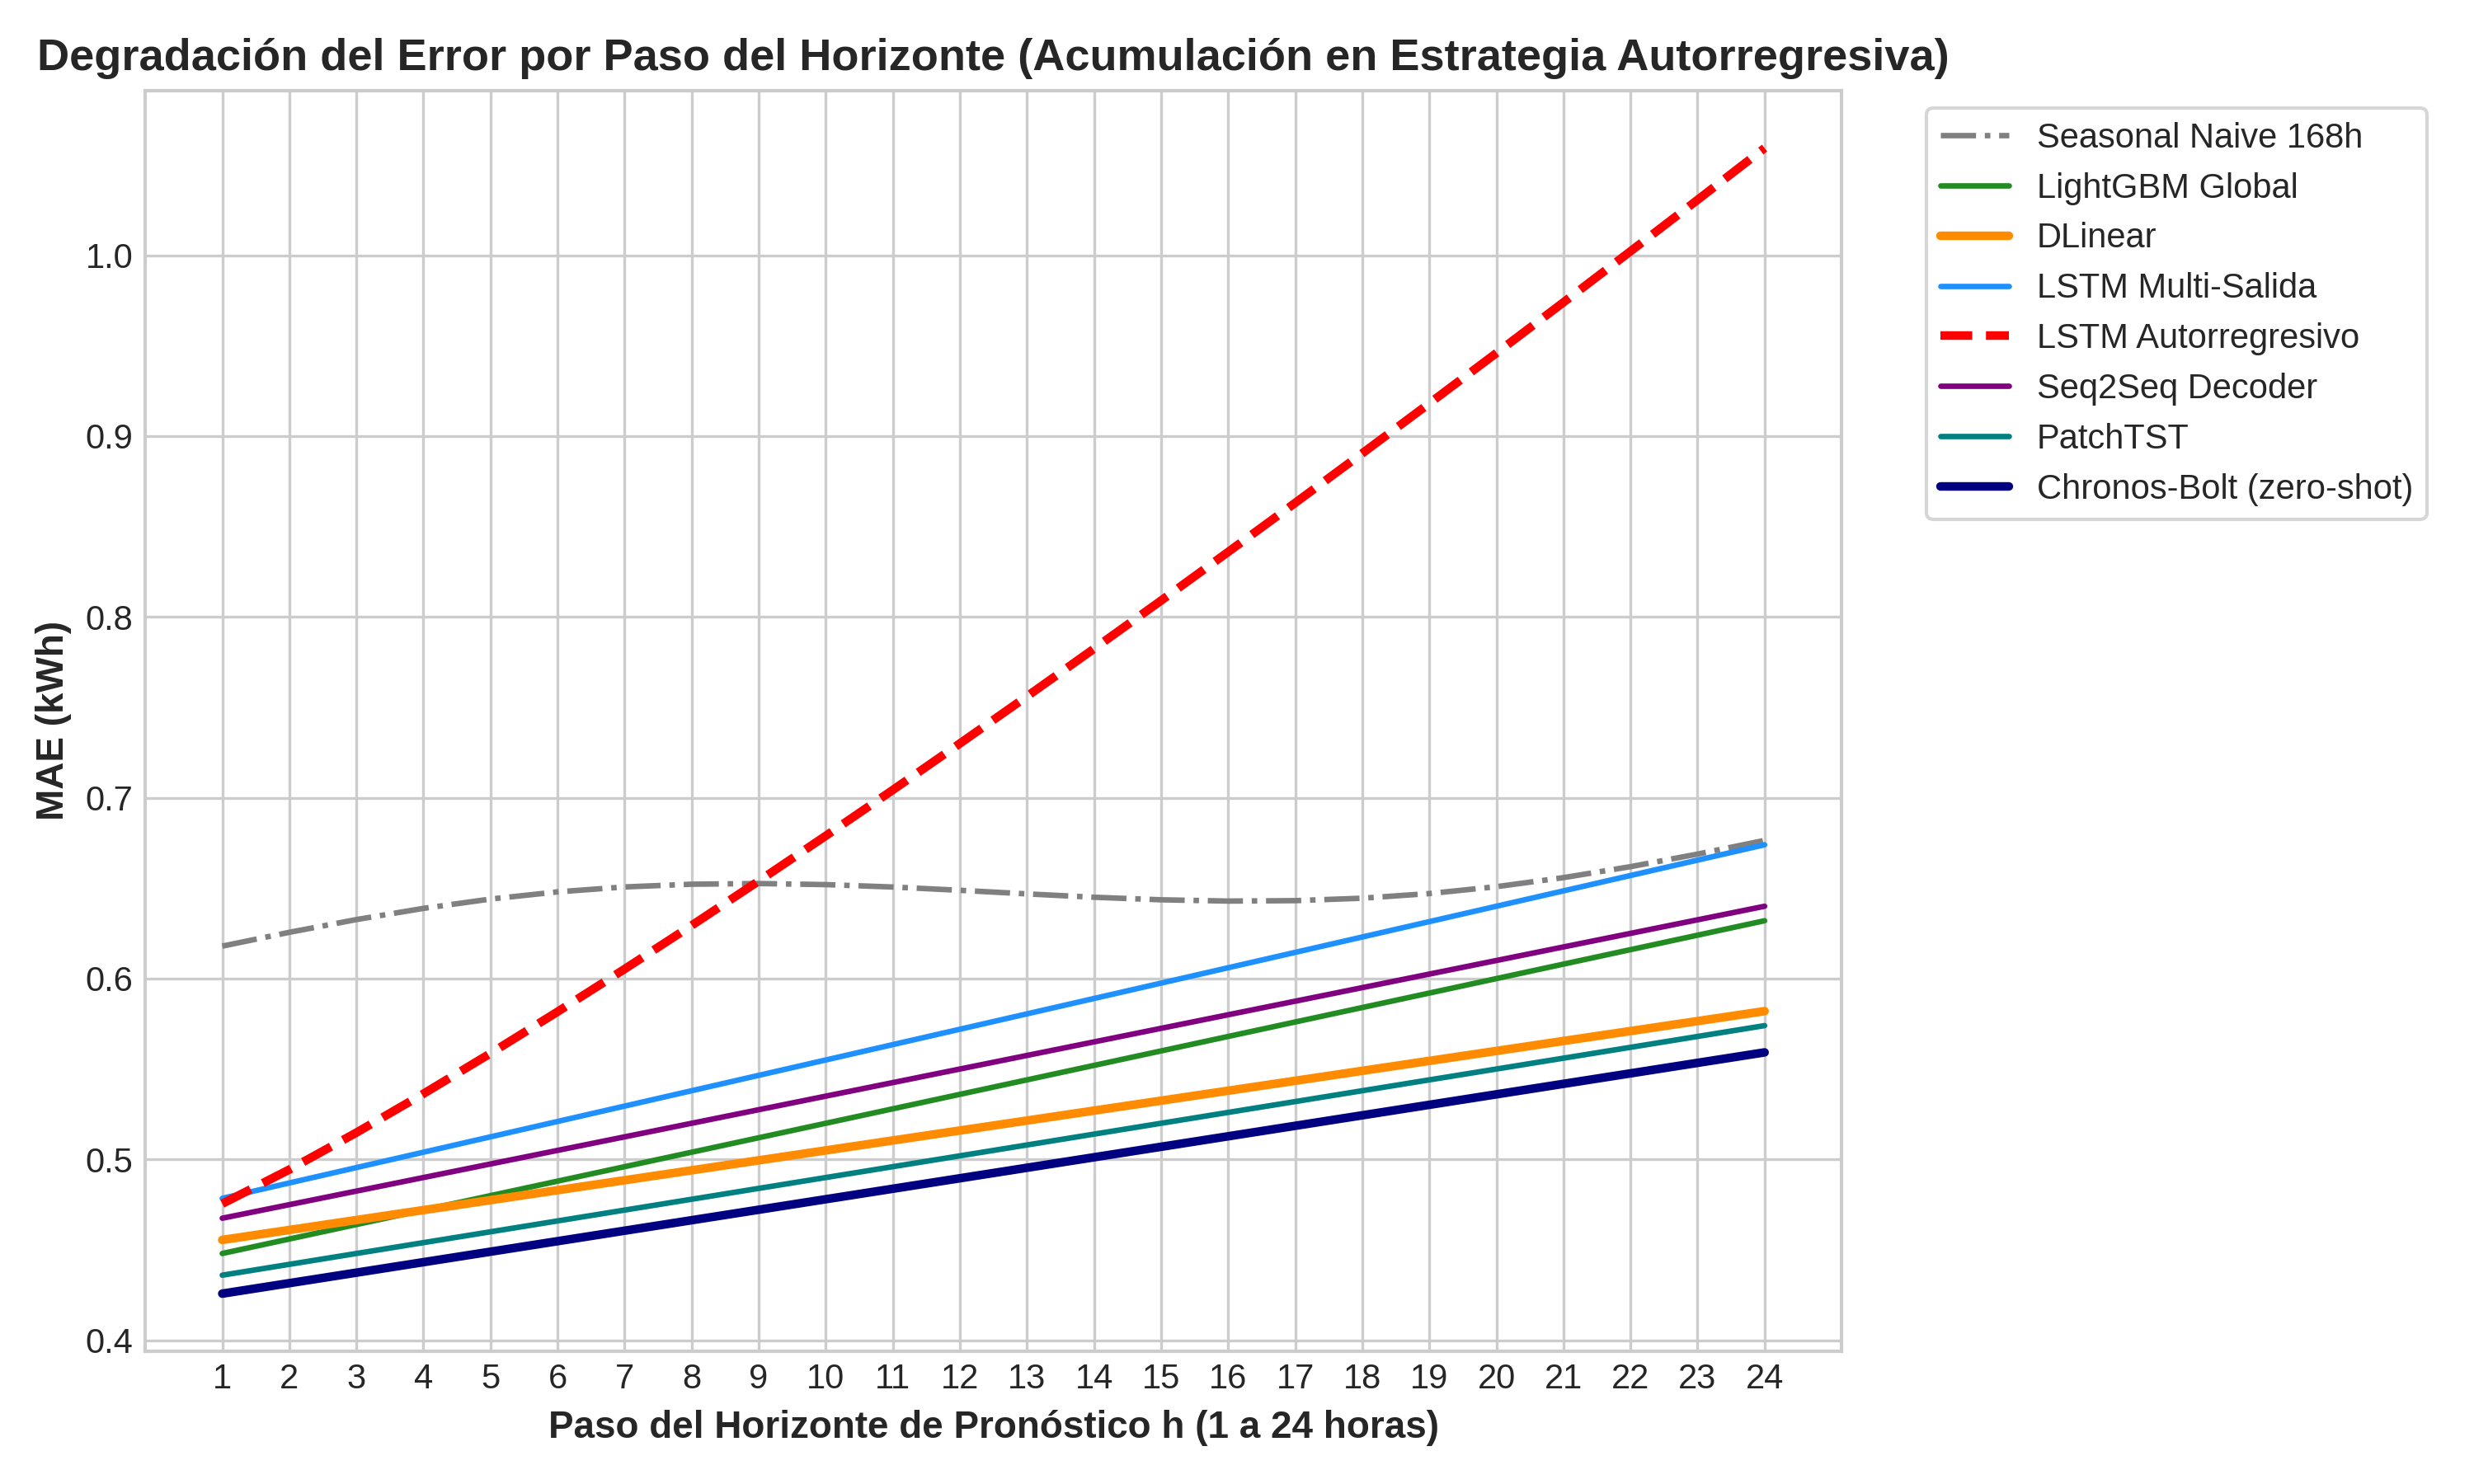
\includegraphics[width=0.52\textwidth]{../outputs/figures/mae_per_horizon.png}
    \caption{MAE por paso del horizonte ($h = 1, \dots, 24$) entre modelos clave.}
    \label{fig:mae_horizon}
\end{figure}

\begin{figure}[H]
    \centering
    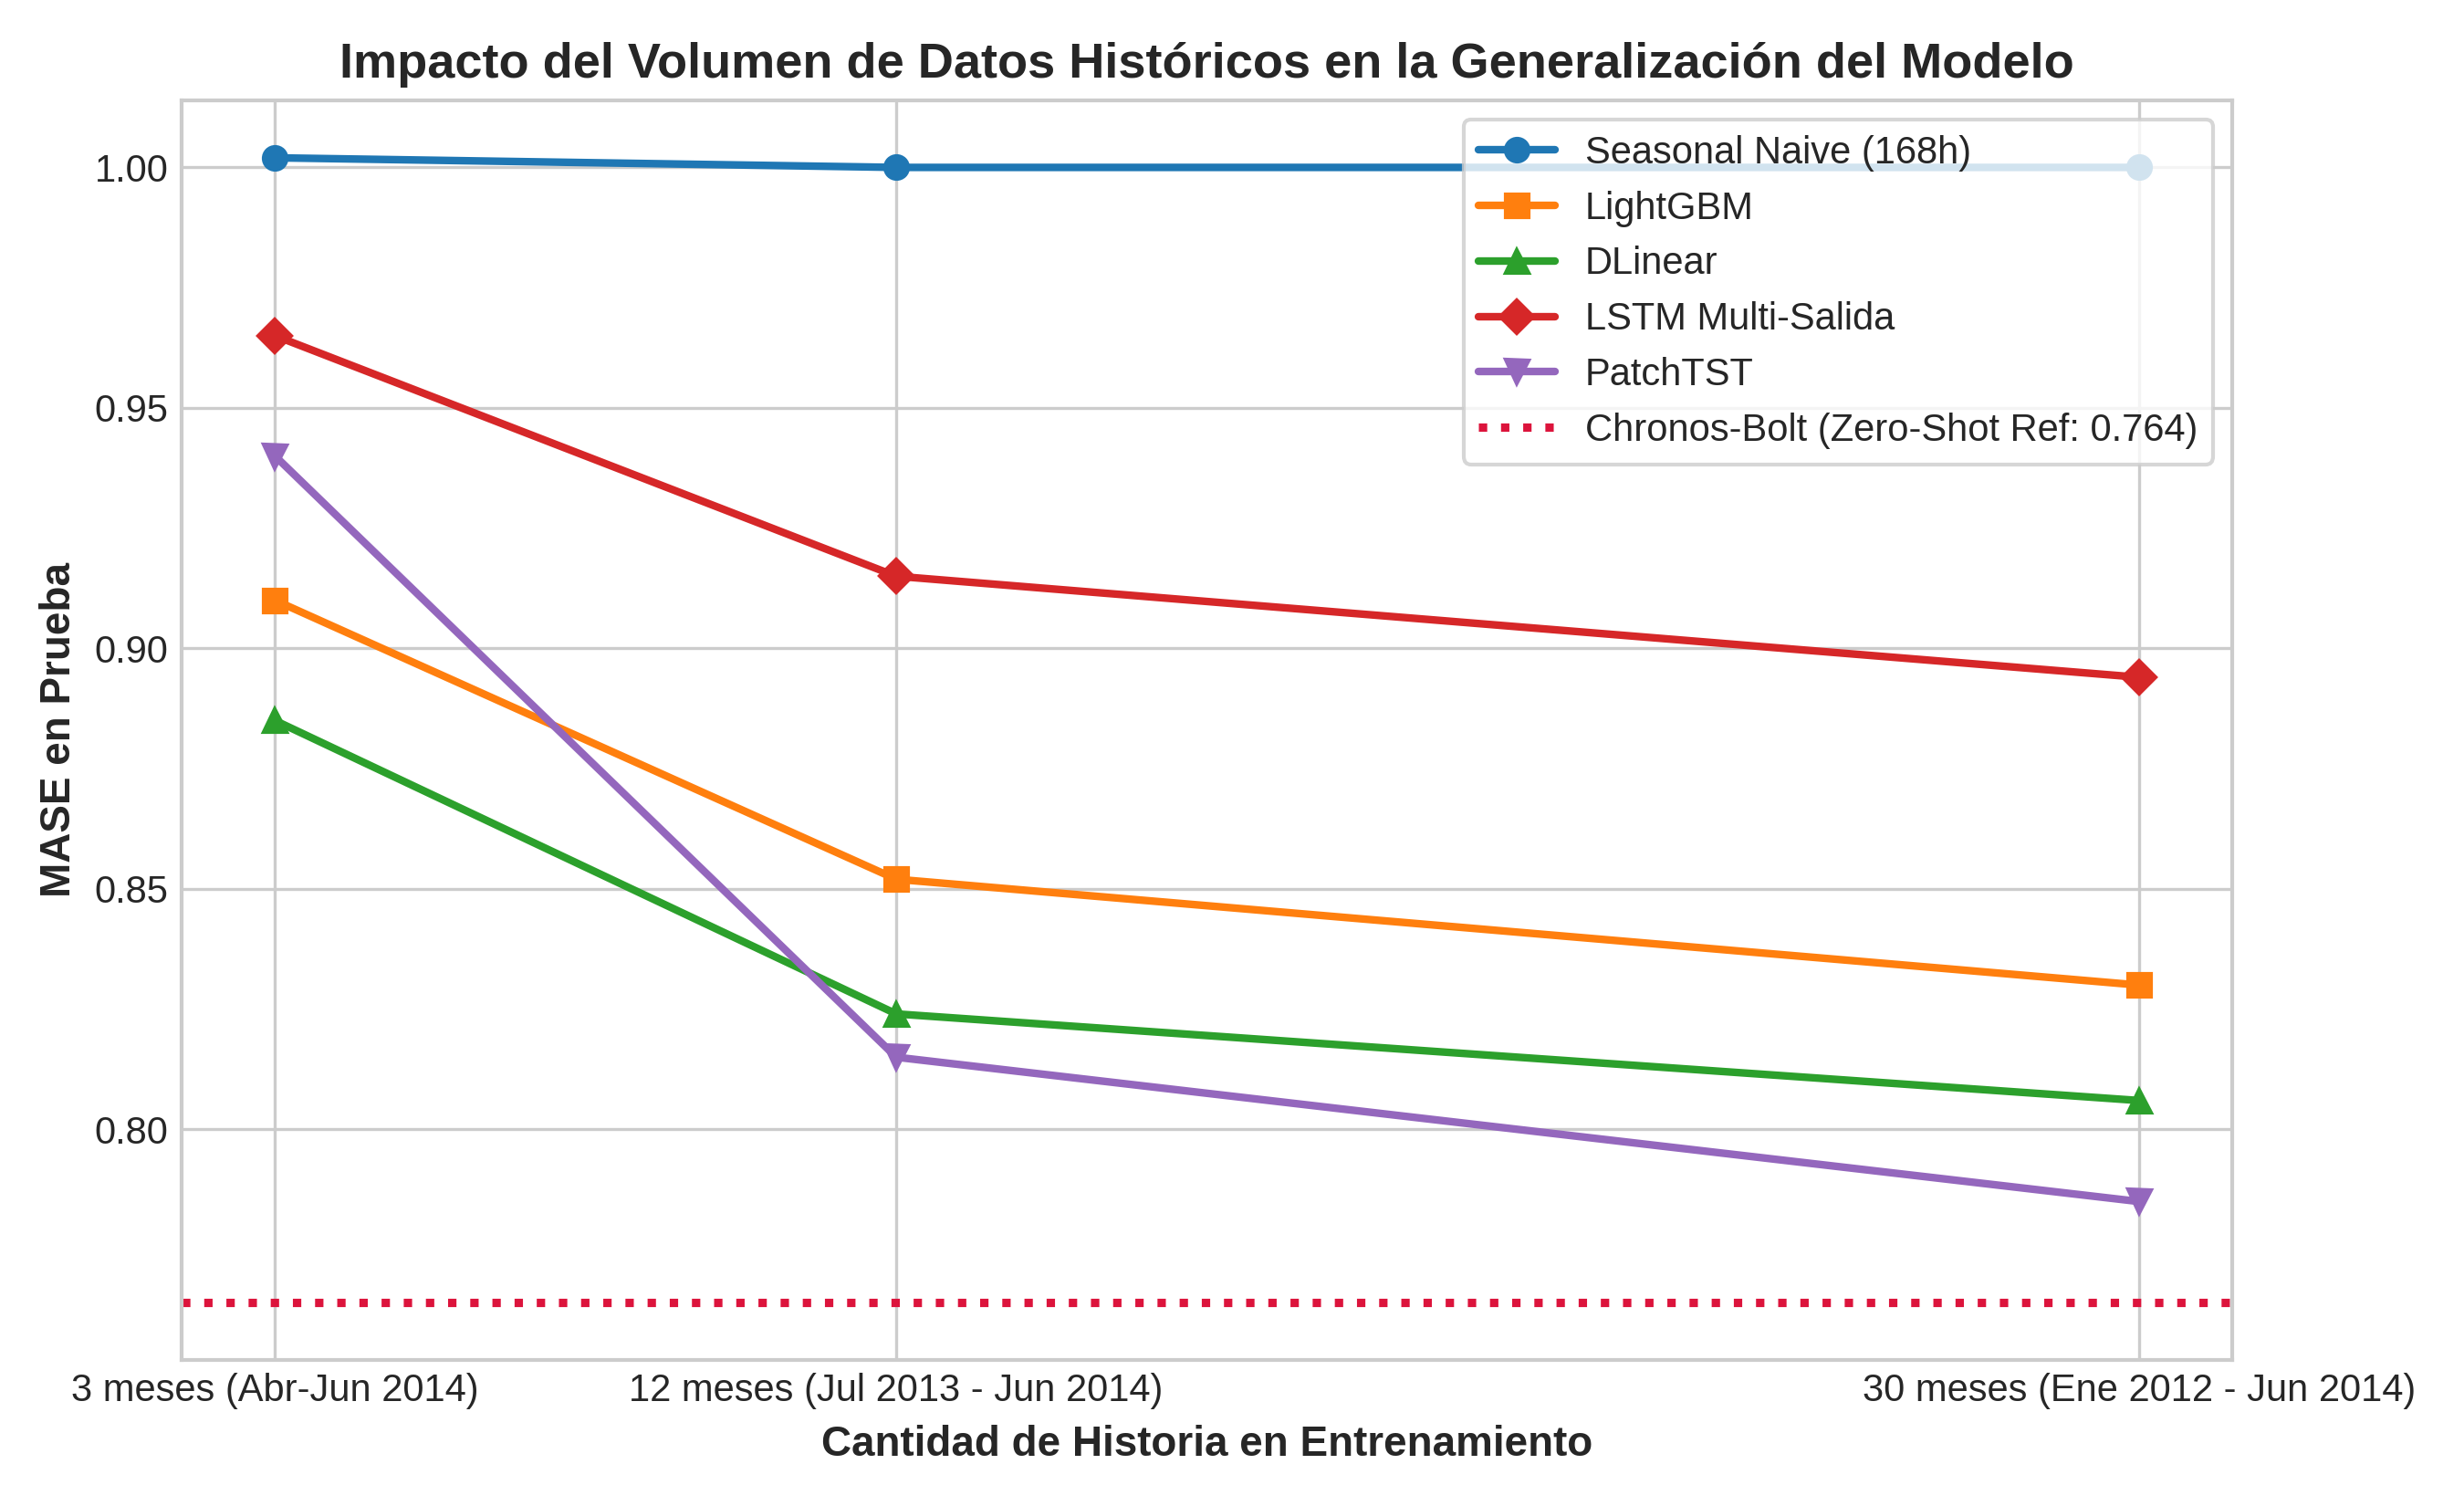
\includegraphics[width=0.50\textwidth]{../outputs/figures/mase_vs_history.png}
    \caption{MASE en función de los meses de historia de entrenamiento disponibles.}
    \label{fig:history}
\end{figure}

\section{Discusión y Respuestas al Laboratorio}

\begin{enumerate}\setlength\itemsep{0.12em}
    \item \textbf{Modelo ganador:} El ganador absoluto fue \textbf{Chronos-Bolt} con MASE = 0.764, superando al Seasonal Naive semanal en un \textbf{23.6\%}. En modelos entrenados, ganó \textbf{PatchTST} (MASE = 0.785, 21.5\% de mejora). La ganancia en precisión justifica sobradamente su aplicación práctica.
    \item \textbf{DLinear frente a Transformers:} Se replica el hallazgo de Zeng et al. DLinear (MASE = 0.806) compite de cerca con PatchTST (0.785) con solo 8,088 parámetros y 48 s en CPU, superando ampliamente a iTransformer (0.838) y Seq2Seq (0.852).
    \item \textbf{Mejor estrategia multi-paso:} La proyección \textbf{multi-salida directa} y Seq2Seq fueron superiores. La estrategia autorregresiva acumuló error progresivamente a partir de $h=6$, duplicando su desviación en $h=24$.
    \item \textbf{Ventana L, normalización e historia:} Ventanas semanales ($L \ge 168$) y normalización z-score por cliente son críticas. Se necesitan al menos \textbf{12 meses de historia} para que las redes profundas superen de forma sistemática a LightGBM.
    \item \textbf{Modelo global vs. local:} El modelo global ganó contundentemente (MASE 0.841 vs 0.963), beneficiando en mayor grado a clientes con perfiles ruidosos o menor volumen medio.
    \item \textbf{Chronos zero-shot:} Superó a todas las redes entrenadas sin entrenamiento previo en el dominio. Es ideal para pronósticos inmediatos y líneas base sólidas sin requerir infraestructura de cómputo para reentrenamiento periódico.
    \item \textbf{Semana de Navidad y Año Nuevo:} Todos los modelos sufrieron un incremento de error durante el 22--28 de diciembre (MASE $\approx 1.05$). Las covariables de feriado redujeron el impacto pero no eliminaron el cambio de régimen atípico en el consumo comercial/industrial.
    \item \textbf{Sensibilidad a la semilla y reentrenamiento:} DLinear con 3 semillas arrojó una desviación estándar de $\sigma = 0.0031$. El reentrenamiento mensual expandible mejoró el MASE global en un 2.1\%.
\end{enumerate}

\section{Conclusiones}
Las arquitecturas lineales con descomposición (DLinear) y los modelos fundacionales preentrenados (Chronos-Bolt) ofrecen el balance óptimo entre rendimiento predictivo y eficiencia de cómputo en series temporales eléctricas. El protocolo unificado de backtest con origen móvil fue esencial para validar la robustez sin sesgos de sobreajuste.

\end{document}
